%%%%%%%%%%%%%%%%%%%% author.tex %%%%%%%%%%%%%%%%%%%%%%%%%%%%%%%%%%%
%
% sample root file for your "contribution" to a contributed volume
%
% Use this file as a template for your own input.
%
%%%%%%%%%%%%%%%% Springer %%%%%%%%%%%%%%%%%%%%%%%%%%%%%%%%%%


% RECOMMENDED %%%%%%%%%%%%%%%%%%%%%%%%%%%%%%%%%%%%%%%%%%%%%%%%%%%
\documentclass[graybox]{svmult}

% choose options for [] as required from the list
% in the Reference Guide

\usepackage{mathptmx}       % selects Times Roman as basic font
\usepackage{helvet}         % selects Helvetica as sans-serif font
\usepackage{courier}        % selects Courier as typewriter font
\usepackage{type1cm}        % activate if the above 3 fonts are
                            % not available on your system
%
\usepackage{makeidx}         % allows index generation
\usepackage{graphicx}        % standard LaTeX graphics tool
                             % when including figure files
\usepackage{multicol}        % used for the two-column index
\usepackage[bottom]{footmisc}% places footnotes at page bottom

% see the list of further useful packages
% in the Reference Guide

\makeindex             % used for the subject index
                       % please use the style svind.ist with
                       % your makeindex program

%%%%%%%%%%%%%%%%%%%%%%%%%%%%%%%%%%%%%%%%%%%%%%%%%%%%%%%%%%%%%%%%%%%%%%%%%%%%%%%%%%%%%%%%%

\usepackage{graphicx}
\usepackage{amsmath}
\usepackage{amssymb}
\usepackage{algorithm}
\usepackage{algorithmic}

\usepackage{amssymb}
\usepackage{amsmath}
\usepackage{xspace}

%\newcommand{\1}{\mathbf{1}}
\newcommand{\dom}{\operatorname{dom}}   
\newcommand{\piecewise}[1]{\left\{ \begin{array}{ll}#1\end{array} \right.}
\newcommand{\argmax}{\operatorname{argmax}}
\newcommand{\argmin}{\operatorname{argmin}}
\newcommand{\mat}[2]{\left[ \begin{array}{#1}#2\end{array} \right]}
\newcommand{\ie}{\textit{i.e.}\xspace}
\newcommand{\eg}{\textit{e.g.}\xspace}
\newcommand{\ip}[1]{\langle #1 \rangle}
%\newcommand{\ipx}[2]{\langle #1, #2 \rangle}
\newcommand{\F}{\mathcal{F}}
\newcommand{\R}{\mathbb{R}}
\renewcommand{\S}{\mathbb{S}}
\renewcommand{\P}{\mathbb{P}}
\renewcommand{\Pr}{\mathbb{P}}
%\newcommand{\E}{\mathbb{E}}
\newcommand{\M}{\mathbb{M}}
\renewcommand{\L}{\mathcal{L}}
\newcommand{\1}[1]{\mathbf{1}\{#1\}}
\newcommand{\sgn}{\mbox{sgn}}
\newcommand{\KL}[2]{\mathbf{KL}\left( #1 \bigg|\bigg| #2 \right)}
\newcommand{\tr}{\textrm{ tr }}
\newcommand{\N}{\mathcal{N}}
\newcommand{\minimize}[1]{\underset{#1}{\mbox{minimize}}\quad}
\newcommand{\maximize}[1]{\underset{#1}{\mbox{maximize}}\quad}
\newcommand{\st}{\mbox{subject to }\quad}
\newcommand{\belbar}{\overline{\operatorname{bel}}}
\newcommand{\bel}{\operatorname{bel}}
\newcommand{\rank}{\operatorname{rank}}
\newcommand{\code}[1]{\begin{verbatim}#1\end{verbatim}}
\newcommand{\todo}[1]{\textcolor{red}{[[#1]]}}
\newcommand{\outline}[1]{\paragraph{#1}}
\newcommand{\tidbit}[1]{\noindent $\mathbf{\bigcirc}$ #1\\}

\newcommand{\vga}{VGA\xspace}
\newcommand{\qqvga}{QQVGA\xspace}


\begin{document}

\title*{Learning to Segment and Track in RGBD}
\author{Alex Teichman, Jake Lussier, and Sebastian Thrun}
\institute{Stanford University}

\maketitle
% \thispagestyle{empty}

%%%%%%%%% ABSTRACT

\newcommand{\thisabs}{
We consider the problem of segmenting and tracking deformable objects in color video with depth (RGBD) data available from commodity sensors such as the Asus Xtion Pro Live or Kinect.  We frame this problem with very few assumptions - no prior object model, no stationary sensor, no prior 3D map - thus making a solution potentially useful for a large number of applications, including semi-supervised learning, 3D model capture, and object recognition.

Our approach makes use of a rich feature set, including local image appearance, depth discontinuities, optical flow, and surface normals to inform the segmentation decision in a conditional random field model.  In contrast to previous work in this field, the proposed method \emph{learns} how to best make use of these features from ground-truth segmented sequences.  We provide qualitative and quantitative analyses which demonstrate substantial improvement over the state of the art.

This paper is an extended version of our previous work \cite{teichman2012a}.  Building on this, we show that it is possible to achieve an order of magnitude speedup and thus real-time performance ($\sim$15FPS) by applying simple algorithmic optimizations to the original work.  This speedup comes at only a minor cost in overall accuracy and thus makes this approach applicable to interactive uses rather than offline only.  Finally, we demonstrate one possible application: efficiently collecting training data for an off-the-shelf object detector.

}

\abstract*{\thisabs}
\abstract{\thisabs}

%%%%%%%%% BODY TEXT
\section{Introduction}
\label{sec:intro}

The availability of commodity depth sensors such as the Kinect opens the door for a number of new approaches to important problems in robot perception.  In this paper, we consider the task of propagating an object segmentation mask through time. It is assumed that a single initial segmentation is given; in this work the initial segmentation is provided by human labeling, but this input could instead come from an automatic method depending on the application.  We do not assume the presence of a pre-trained object model (\ie as the Kinect models human joint angles), as that would preclude the system from segmenting and tracking arbitrary objects of interest.  As such, this task falls into the category of \emph{model-free} segmentation and tracking, \ie no prior class model is assumed.  Similarly, we do not assume the sensor is stationary or that a pre-built static environment map is available.  As ``model-free segmentation and tracking'' is somewhat unwieldy, we will sometimes refer to this task as STRGEN (sturgeon), for ``segmentation and tracking of generic objects''. \todo{Not settled on a name yet, but need something.  Happy to hear suggestions.}

\begin{figure}
  \centering
  \includegraphics[width=\linewidth]{img/mfst.pdf}
  \caption{Definition of the model-free segmentation and tracking task which this paper addresses.  Given an initial seed labeling (first frame; cat on a coffee table), the goal is to produce a detailed segmentation of the object over time (subsequent frames) without assuming the existence of a pre-trained object model.  Foreground points are shown bold and colored, background small and gray.}
  \label{fig:goal}
\end{figure}


\subsection{Example use cases and long-term vision}
\label{sec:examples}

There are several reasons a complete solution to the STRGEN task would be useful in robotics, computer vision, and graphics.  For example, this would make possible a generic and and natural object selection interface which could be used for 3D model capture in unstructured environments.  In the following, however, we will focus primarily on the area of object recognition.

\subsubsection{Training data collection for standard object detectors}
\label{sec:trainingintro}

Much work has been put into object detection methods using RGBD sensors.  While off-the-shelf object detections algorithms such as LINE-MOD \cite{hinterstoisser2011a} are often fast and effective at runtime, the collection of training data remains a hassle.  Typical approaches include turntables and crowdsourcing.  While the former allows for high-quality training examples for a full $360^{\circ}$ range of views, it also involves an appropriate rig, is limited to objects that can be easily placed in a rig, and must be repeatedly reconfigured for different perspectives.  The latter allows for unstructured environments and avoids the physical setup annoyances but also requires a well-designed web application and a data processing framework robust to noisy and incompatible responses. This approach is also altogether inapplicable for problems involving sensitive data.  Other data labeling approaches, such as learning and subtracting a background model, are rare as they are generally slower to collect significant quantities of training data for objects that do not move on their own.

Model-free segmentation and tracking enables training data collection which eliminates these disadvantages.  Using a handheld depth sensor and tablet, training data can be collected in unstructured environments by taking sparse labeling hints from the user and generating segmentations over time, providing new training examples with different object poses, view angles, lighting conditions, and so on, with little additional human effort.  A prototype of such a system is shown in Figure~\ref{fig:usage}; see also Section~\ref{sec:example} for an experiment using a similar concept.

\begin{figure}
  \centering
  \includegraphics[width=\linewidth]{img/usage-smaller.pdf}
  \caption{Example usage of model-free segmentation and tracking algorithm for object detector training set collection.  Initially, no object is being tracked.  A user provides sparse foreground and background hints as the RGBD data streams in.  Segmented objects are shown in red. \todo{Show pose changes, fix focus}}
  \label{fig:usage}
\end{figure}

As shown in Section~\ref{sec:example}, this application example is currently practical.  The examples that follow likely require improvements in segmentation accuracy or other research progress to become practical, but the obstacles in the path are probably not insurmountable.

\subsubsection{Track classification}

Currently, most object recognition methods fall into semantic segmentation or sliding window categories.  When a solution to the STRGEN problem is available, however, it is possible to use a different approach, exemplified in \cite{teichman2011a}.  In this approach, objects are segmented and tracked over time without a semantic label and the track as a whole is classified online as new segmented frames stream in; we refer to this object recognition problem breakdown as STAC, for segmentation, tracking, and classification.  As shown in \cite{teichman2011a}, the STAC approach significantly improves classification accuracy because of its ability to use multiple views over time and to use track descriptors such as average object speed or maximum angular velocity.  In \cite{teichman2011a}, model-free segmentation and tracking was available due to the specific circumstances of autonomous driving that are not generally applicable.  A solution to the general model-free segmentation and tracking problem, however, would enable this approach in less structured environments.

\subsubsection{Tracking-based semi-supervised learning}

A solution to the STAC problem opens the door to a simple and effective method of semi-supervised learning in which a large number of unlabeled tracks of objects are used in conjunction with a small number of hand-labeled tracks to learn an accurate classifier.  This method, known as tracking-based semi-supervised learning (TBSSL), was demonstrated in the autonomous driving context using laser range finders to learn to accurately recognize pedestrians, bicyclists, and cars versus other distractor objects in the environment using very few hand-labeled training examples \cite{teichman2011b}. However, as with \cite{teichman2011a}, model-free segmentation and tracking was more or less freely available because objects on streets generally avoid collision and thus remain depth-segmentable using simple algorithms.  To extend tracking-based semi-supervised learning to the more general case in which objects are not easily depth-segmentable, a more general solution to the STRGEN problem is required.

\subsubsection{Long-term vision}

The primary long-term motivation for this work is to enable object recognition systems that produce high-quality results, yet are trainable and usable by regular people using only modest amounts of effort. The success of STAC and TBSSL given model-free segmentation and tracking hint that this may be possible.  One option is to A) collect a small number of training examples using a natural interface such as that of Figure~\ref{fig:usage}, B) apply TBSSL to learn a high-quality classifier from large quantities of unlabeled data, and C) run STAC to recognize objects using the learned classifier.  The primary missing component in this system or variations thereof is a high-accuracy and real-time solution to the general STRGEN problem.

\section{Previous work}
\label{sec:prev_work}
\todo{maybe move this to the end so comparisons of our method with others are easier to follow}

While there is much previous work on tracking in general, our problem's online nature, output of detailed segmentation masks rather than bounding boxes, and lack of simplifying assumptions restrict the directly-related previous work substantially.  The most similar and recent work to ours is HoughTrack \cite{godec2011a}, which uses Hough Forests and GrabCut to segment consecutive frames.  We provide a quantitative comparison to HoughTrack in Section~\ref{sec:quant}.  Older previous work on this problem include \cite{bibby2008a} and their multi-object extension \cite{bibby2010a}, which use a generative model and level sets; \cite{kwon2009a}, which tracks local object patches using Basin Hopping Monte Carlo sampling; and \cite{ren2007a}, which uses a conditional random field model and loopy belief propagation. All these works limit themselves to only a small number of features and do not use learning methods to find the best general-purpose tracker.  Additionally, none of these works consider depth information.

We now briefly review previous work on related problems.

\textbf{Interactive segmentation} - Human-assisted object segmentation has been the subject of much work including interactive graph cuts \cite{boykov2001a}, GrabCut \cite{rother2004a}, and Video SnapCut \cite{bai2009a}.  These methods are largely intended for graphics or assisted-labeling applications as they require a human in the loop.  This paper addresses automatic segmentation with the exception of the application example in Section~\ref{sec:example}.

\textbf{Bounding box tracking} - Discriminative tracking \cite{grabner2006a, stalder2009a, kalal2010a} addresses the online, model-free tracking task, but where the goal is to track arbitrary objects in a bounding box rather than provide a detailed segmentation mask.

\textbf{Rigid object tracking} - Rigid object tracking using depth information, such as the open source method in PCL \cite{rusu2011a}, addresses a similar but simpler problem, as it is not designed to work with deformable objects.

\textbf{Offline methods} - The work of \cite{budvytis2011a} takes as input segmentations for the first and last frames in a sequence, rather than just the first frame.  While \cite{tsai2010a} takes as input only the segmentation of the first frame, they construct a CRF on the entire video sequence, with CRF labels corresponding to object flows.  Here we are interested in a method that can update as new data streams in, thus making it applicable for robotics or other online vision tasks.

\textbf{Background subtraction} - Background subtraction approaches can greatly simplify the segmentation task.  For example, \cite{aeschliman2010a} assumes a stationary camera to produce fine-grained segmentation masks for multiple objects.  With depth sensors, background subtraction methods can also operate while the sensor is in motion: Google's autonomous car project uses pre-built 3D static environment maps to subtract away all 3D points except the moving obstacles \cite{urmson2011a}.  This enables simple depth segmentation to be effective as long as moving objects do not touch, but assumes a high-precision localization system as well as a pre-learned static environment map.

\textbf{Model-based tracking} - For some tasks, it is appropriate to model a specific object that is to be tracked, either with an explicit 3D model as in \cite{prisacariu2009a} or with pre-trained statistical models that are specific to the particular object class.  Examples of the latter approach include the human pose tracking of the Kinect \cite{shotton2011a} and model-based car tracking in laser data for autonomous driving \cite{petrovskaya2009a}.

It is worth noting that the line between model-free and model-based tracking is not sharp.  Because several of our intended applications revolve around training detectors for previously-unseen objects, we restrict ourselves to making use of object models that are learned on the fly.  It is entirely conceivably, however, that one could plug in a detailed pre-trained object model to our framework to produce higher accuracy results for that particular object.

\section{Approach}

There are a large number of possible cues that could inform a segmentation and tracking algorithm.  Optical flow, image appearance, 3D structure, depth discontinuities, color discontinuities, etc., all provide potentially useful information.  For example:
\begin{itemize}
  \item An optical flow vector implies that the label of the source pixel at time $t-1$ is likely to propagate to that of the destination pixel at time $t$.
\item Pixels with similar color and texture to previous foreground examples are likely to be foreground.
\item The shape of the object in the previous frame is likely to be similar to the shape of the object in the next frame.
\item Points nearby in 3D space are likely to share the same label.
\item Nearby points with similar colors are likely to share the same label.
\end{itemize}

Previous work generally focuses on a few particular features; here, we advocate the use of a large number of features.  The above intuitions can be readily encoded by node and edge potentials in a conditional random field model.  However, this additional complexity introduces a new problem: how much importance should each feature be assigned?  While using a small number of features permits their weights to be selected by hand or tested with cross validation, this quickly becomes impractical as the number of features increases.

The margin-maximizing approach of structural SVMs \cite{taskar2005a, tsochantaridis2005a}, adapted to use graph cuts for vision in \cite{szummer2008a}, provides a solution to learning in these scenarios.  Intuitively, this method entails running MAP inference, and then adding constraints to an optimization problem which assert that the margin between the ground truth labeling and the generated (and generally incorrect) labeling should be as large as possible.  The application of this approach will be discussed in detail in Section~\ref{sec:learning}.


\subsection{Conditional random fields and inference}
\label{sec:inference}

A conditional random field is an undirected graphical model that can make use of rich feature sets and produce locally-consistent predictions.  It aims to spend modeling power on only the distribution of the target variables given the observed variables.  In particular, the conditional random field takes the form
\begin{align}
  \Pr(y | x) = \frac{1}{Z(x)} \exp(-E(y, x)),
\end{align}
where $Z$ is the normalizer or partition function, $y~\in~\{-1,+1\}^n$ is the segmentation for an image with $n$ pixels, and $x$ is a set of features defined for the RGBD frame, to be detailed later.  The energy function $E$ contains the features that encode various intuitions about what labels individual pixels should take and which pixels should share the same labels.  In particular, the energy function is defined as
\begin{align}
  E(y, x) = & \sum_{i \in \Phi_\nu} w_i \sum_{j \in \nu_i} \phi_j^{(i)}(y, x) \label{eqn:energy} + \sum_{i \in \Phi_{\mathcal{E}}} w_i \sum_{(j,k) \in \mathcal{N}_i}  \phi_{jk}^{(i)}(y, x).
\end{align}
Here, $\Phi_\nu$ is the set of node potential indices (\ie one for each type of node potential such as local image appearance or 3D structure alignment), $\nu_i$ is the set of all node indices for this potential type (normally one per pixel), and $\phi_j^{(i)}$ is the node potential of type $i$ at pixel $j$.  Similarly, $\Phi_\mathcal{E}$ is the set of edge potential indices, $\mathcal{N}_i$ is the neighborhood system for edge potential type $i$ (normally pairs of neighboring pixels), and $\phi_{jk}^{(i)}$ is the edge potential between pixels $j$ and $k$ for edge potentials of type $i$.  Thus, the weights apply at the feature-type level, \ie $w_i$ describes how important the $i$th feature is.

The goal of MAP inference in this model is to choose the most likely segmentation $y$ given the features $x$ by solving
\begin{align}
  \maximize{y} \Pr(y | x) = \minimize{y} E(y, x).
\end{align}
During inference, the weights $w$ remain fixed.  The solution to this problem can be efficiently computed for $y \in \{-1, +1\}^n$ and submodular energy function $E$ using graph cuts \cite{boykov2001a}.

\subsection{Learning}
\label{sec:learning}

Given a dataset of $(y_i, x_i)$ for $i=1 \dots m$, the goal of CRF learning is to choose the weights $w$ that will result in the lowest test error. While it would be desirable to learn the weights directly using the maximum likelihood approach
\begin{align}
  \maximize{w} \prod_m \Pr(y_m | x_m),
\end{align}
this is not possible to do exactly because of the presence of the partition function $Z(x) = \sum_{y} \exp(-E(y, x))$ in the gradient.  This function sums over all $2^n$ segmentations of an image with $n$ pixels.
  
Fortunately, there is an alternative approach known as the structural support vector machine \cite{taskar2005a, tsochantaridis2005a, szummer2008a}, which we now briefly review.  Solving the margin maximizing optimization problem
\begin{equation}
  \begin{aligned}
    & \minimize{w, \xi} & & \frac{1}{2} ||w||^2 + \frac{C}{M} \sum_{m=1}^M \xi_m \label{eqn:nslack} \\
    & \st & & \xi \geq 0 \\
& & & E ( y, x_m ) - E ( y_m, x_m ) \geq \Delta (y_m, y) - \xi_m \quad \forall m, \forall y \in \mathcal{Y}
  \end{aligned}
\end{equation}
would result in a good solution. Here, $C$ is a constant, $\Delta$ is a loss function, $\xi_m$ is a slack variable for training example $m$, and $\mathcal{Y}$ is the set of all possible labelings of an image. This problem, too, is intractable because it has exponentially many constraints.  However, one can iteratively build a small, greedy approximation to the exponential set of constraints such that the resulting weights $w$ are good.

Further, one can transform (\ref{eqn:nslack}), known as the $n$-slack formulation, into the equivalent problem
\begin{equation}
  \begin{aligned}
    & \minimize{w, \xi} & & \frac{1}{2} ||w||^2 + C\xi \\
    & \st & & \xi \geq 0 \\
    & & & \frac{1}{M} \sum_{m=1}^M E ( \hat{y}_m, x_m )
    - E ( y_m, x_m ) \geq \frac{1}{M} \sum_{m=1}^M \Delta(y_m, \hat{y}_m) - \xi \\
    & & & \quad \forall (\hat{y}_1, ..., \hat{y}_M) \in \mathcal{Y}^M,
  \end{aligned}
\end{equation}
as described in \cite{joachims2009a}.  As before, while the number of constraints is exponential, one can build a small, greedy approximation that produces good results.  Known as the 1-slack formulation, this problem is equivalent and can be solved much more efficiently than (\ref{eqn:nslack}), often by one or two orders of magnitude.

The goal is to learn the weights that will best segment an entire sequence given a single seed frame.  However, the segmenter operates on a single frame at a time, so our training dataset must be in the form of $(y, x)$ pairs. As will be discussed in Section~\ref{sec:energy}, some of the features are stateful, \ie they depend on previous segmentations.  This presents a minor complication.  At training time, we do not have access to a good choice of weights $w$, but the features depend on previous segmentations which in turn depend on the weights.  To resolve this, we adopt the simple strategy of generating features assuming that previous segmentations were equal to ground truth.  This dataset generation process is specified in Algorithm~\ref{alg:dataset}.

\begin{algorithm}
  \caption{Training set generation}
  \label{alg:dataset}
  \begin{algorithmic}
    \STATE $\mathbb{S} = \{S : S = ((y_0, d_0), (y_1, d_1),                       \dots)\}$ is a set of sequences,
\STATE $\qquad$ where $y_i$ is a ground truth segmentation and $d_i$ is an RGBD frame
\STATE $\mathcal{D} = \emptyset$
\FOR{$S \in \mathbb{S}$}
\STATE Initialize stateful components, \eg the patch classifier that learns its model online
\FOR{$(y_i, d_i) \in S$}
\STATE Update stateful components using $y_{i-1}$ as the previous segmentation
\STATE Generate features $x$
\STATE $\mathcal{D} := \mathcal{D} \cup \{(y_i, x)\}$
\ENDFOR
\ENDFOR
\RETURN $\mathcal{D}$
  \end{algorithmic}
\end{algorithm}

\begin{algorithm}[h]
  \caption{Structural SVM for learning to segment and track}
  \label{alg:ssvm}
  \begin{algorithmic}
    \STATE $\mathcal{D}$ is a set of training examples $(y, x)$,                             formed as described in Algorithm~\ref{alg:dataset}.
\STATE $C$ and $\epsilon$ are constants, chosen by cross validation.
\STATE 
\STATE $\mathcal{W} \leftarrow \emptyset$
\REPEAT
\STATE Update the parameters $w$ to maximize the margin.
\begin{equation*}
  \begin{aligned}
    & \minimize{w, \xi} & & \frac{1}{2} ||w||^2 + C\xi \\
    & \st & & w \geq 0, \quad \xi \geq 0 \\
    & & & \frac{1}{M} \sum_{m=1}^M E ( \hat{y}_m, x_m )
    - E ( y_m, x_m ) \geq \frac{1}{M} \sum_{m=1}^M \Delta(y_m, \hat{y}_m) - \xi \\
    & & & \quad \forall (\hat{y}_1, ..., \hat{y}_M) \in \mathcal{W}
  \end{aligned}
\end{equation*}

\FOR{$( y_m, x_m ) \in \mathcal{D}$}
\STATE Find the MAP assignment using graph cuts.
\STATE $\hat{y}_m \leftarrow \argmin_y E (y, x_m )$
\ENDFOR
\STATE $\mathcal{W} \leftarrow \mathcal{W} \cup \{(\hat{y}_1, \dots, \hat{y}_M\}$
\UNTIL $\quad \frac{1}{M} \sum_{m = 1}^M \Delta(y_m, \hat{y}_m) - E ( \hat{y}_m, x_m) + E ( y_m, x_m ) \leq \xi + \epsilon$
  \end{algorithmic}
\end{algorithm}

The structural SVM solver is detailed in Algorithm~\ref{alg:ssvm}.  Because the graph cuts solver assumes a submodular energy function, non-negative edge weights $w_i$ for all $i \in \Phi_{\mathcal{E}}$ are required.  As our node potentials are generally designed to produce values with the desired sign, we constrain them in Algorithm~\ref{alg:ssvm} to have non-negative weights as well.  The term $\Delta (y_m, y)$ is 0-1 loss, but a margin rescaling approach could easily be obtained by changing $\Delta$ to Hamming loss and making a small modification to the graph cuts solver during learning (see \cite{szummer2008a}). 

\subsection{Energy function terms}
\label{sec:energy}

\begin{figure*}
  \centering
  \includegraphics[width=\linewidth]{img/features1.pdf}
  \caption{Visualizations of selected edge and node potentials in the CRF.  Edge potentials are zoomed in to show fine structure.  Strong edge potentials are darker, while weaker edge potentials fade to original image color.  Node potentials expressing a preference for foreground are shown in red, for background in green, and for neither in black.  Top row: original image, canny edge potentials, color distance, depth edge potentials.  Bottom row: ICP, frame alignment bilateral filter, optical flow, and patch classifier node potentials.  Best viewed in color.}
  \label{fig:features}
\end{figure*}

We now review the particular choice of energy function (\ref{eqn:energy}) that we use in our implementation. The particular choice of features can be modified or added to without substantially changing the underlying framework. See Figure~\ref{fig:features} for visualizations.  All node potentials are designed to be constrained to $[-1, +1]$, and all edge potentials to $[-1, 0]$.  While not strictly necessary, this aids in interpreting the weights learned by the structural SVM.

\subsubsection{Node potentials}
\label{sec:npot}
Node potentials capture several aspects of shape, appearance, and motion.  All take the form
\begin{align}
  \label{eqn:npot}
  \phi_j(y, x) = 
  \left\{
  \begin{array}{rl}
    a_j & \mbox{ if } y_j = 1 \\
    b_j & \mbox{ if } y_j = -1,
  \end{array} 
  \right.
\end{align}
where $a_j$ and $b_j$ are functions of the data $x$, and $y_j = 1$ indicates that pixel $j$ has been assigned to the foreground.

\textbf{Seed labels} - The first frame of every sequence provides a foreground/background segmentation.  Seed labels can also be used for algorithm-assisted human labeling, used here only in construction of the ground truth dataset.  Each pixel in the image can be labeled by the user as foreground or background, or left unlabeled.  Concretely, let $s_j \in \{-1,0,+1\}$ be the seed labels for each pixel.  Then, the potential is defined by
\begin{align*}
  \phi_j(y, x) & =
  \left\{
  \begin{array}{rl}
    -1 & \mbox{ if } y_j = s_j \\
    0 & \mbox{ otherwise.}
  \end{array}
  \right.
\end{align*}

\textbf{Optical flow} - Pixels in the current frame with optical flow vectors from the previous frame are likely to have the label of the originating pixel.  If no optical flow vector terminates at pixel $j$ in the current frame, let $f_j = 0$.  Otherwise, let $f_j$ be equal to the label of the originating pixel from the previous frame.  Then, the potential is defined by
\begin{align*}
  \phi_j(y, x) & =
  \left\{
  \begin{array}{rl}
    -1 & \mbox{ if } y_j = f_j \\
    0 & \mbox{ otherwise.}
  \end{array}
  \right.
\end{align*}

\textbf{Frame alignment bilateral filter} - Optical flow provides correspondences from one frame to the next; after aligning these frames, a bilateral filter given 3D position and RGB values is used to blur the labels from the previous frame into the current frame, respecting color and depth boundaries.

Specifically, alignment between the two frames is found using a RANSAC method, with 3D correspondences given by optical flow vectors.  Flow vectors that originate or terminate on a depth edge are rejected, as their 3D location is often unstable.  After alignment, we find the set of neighboring points $N$ from the previous frame within a given radius of the query point, then compute the value
\begin{align*}
  z_j = \sum_{k \in N} y_k' \exp \left(-\frac{||c_j - c_k||_2}{\sigma_c} - \frac{||p_j - p_k||_2}{\sigma_d} \right),
\end{align*}
where $y_k'$ is the $\{-1, +1\}$ label of point $k$ in the previous segmentation, $c_j$ is the RGB value of pixel $j$, and $p_j$ is the 3D location of pixel $j$. The two $\sigma$s are bandwidth parameters, chosen by hand.  The value $z_j$ is essentially that computed by a bilateral filter, but without the normalization.  This lack of normalization prevents a point with just a few distant neighbors from being assigned an energy just as strong as a point with many close neighbors. Referring to (\ref{eqn:npot}), the final energy assignment is made by setting $b_j = 0$ and $a_j = 1 - 2 / (1 + e^{-z_j})$.

\textbf{Patch classifiers} - Two different parameterizations of a random fern patch classifier similar to \cite{ozuysal2007a} are trained online and used to make pixel-wise predictions based on local color and intensity information.

A random fern classifier is a semi-naive Bayes method in which random sets of bit features are chosen (``ferns''), and each possible assignment to the bit features in the fern defines a bin.  Each of these bins maintains a probability estimate by simple counting.  The final probability estimate is arrived at by probabilistically combining the outputs of many different randomly generated ferns.  See \cite{ozuysal2007a} for details.  We use 50 randomly generated ferns, each of which have 12 randomly generated features.

Each bit feature in a fern is generated by very simple functions of the data contained in the image patch.  For example, one of the bit features we use is defined by
\begin{align*}
  z =
  \left\{
  \begin{array}{rl}
    1 & \mbox{ if } I_{p_0} < I_{p_1} \\
    0 & \mbox{ otherwise, }
  \end{array}
  \right.
\end{align*}
where $p_0$ and $p_1$ are two pre-determined points in the image patch, and $I_p$ is the intensity of the camera image at point $p$.  Other bit features include color comparisons and Haar wavelet comparisons, efficiently computed using the integral image.

At each new frame, the classifier is updated using the graph cuts segmentation output from the previous frame as training data, then is used to compute a probability of foreground estimate for every pixel in the current frame. The value $a_j$ is set to the probability of background, and $b_j$ to probability of foreground.

\textbf{Distance from previous foreground} - Points very far away from the object's position in the previous frame are unlikely to be foreground.

After alignment of the current frame to the previous frame using the same optical-flow-driven method as the bilateral term, we compute the distance $d$ from the point $j$ in the current frame to the closest foreground point in the previous frame.  The final potentials are set to $a_j = 0$ and $b_j = \exp(-d / \sigma) - 1$.

\textbf{ICP} - The iterative closest point algorithm is used to fit the foreground object's 3D points (and nearby background points) from the previous frame to the current frame.  If the alignment has a sufficient number of inliers, points in the current frame are given node potentials similar to those of the bilateral node potential, but where the ICP-fit points are used instead of the entire previous frame.

\textbf{Prior term} - To express a prior on background, we add a term for which $a_j = 0$ and $b_j = -1$.

\subsubsection{Edge potentials}

\begin{figure}
  \includegraphics[width=7cm]{img/normals.pdf}
  \sidecaption[t]
  \caption{While image appearance and depth information may sometimes provide little information about an object boundary, a change in surface normals can be informative. Surface normals are shown as small dark lines, seen from two angles to aid in depth perception.}
  \label{fig:normals}
\end{figure}

Edge potentials capture the intuition that the foreground/background boundary is likely to be at an image gradient, color change, depth discontinuity, or surface normal change.  All take the form
\begin{align*}
  \phi_{jk}(y, x) =
  \left\{
  \begin{array}{rl}
    a_{jk} & \mbox{ if } y_j = y_k \\
    0 & \mbox{ otherwise,}
  \end{array}
  \right.
\end{align*}
where $a_{jk}$ is a function of the data $x$.  All edges are between neighboring points in the image.

\textbf{Canny edges} - All neighboring pixels are connected by an edge potential except those cut by canny edges.  Concretely,
\begin{align*}
  a_{jk} & =
  \left\{
  \begin{array}{rl}
    -1 & \mbox{ if neither pixel lies on a Canny edge} \\
    0 & \mbox{ otherwise.}
  \end{array}
  \right.
\end{align*}

%$a_{jk}$ is -1 if neither pixel lies on a Canny edge and is 0 otherwise.

\textbf{Color distance} - Edge weights are assigned based on Euclidean distance between neighboring RGB values; $a_{jk} = - \exp(-||c_j - c_k|| / \sigma)$, where $c_j$ and $c_k$ are the RGB values of the two pixels and $\sigma$ is a bandwidth parameter, chosen by hand.

\textbf{3D distance} - Points nearby in 3D are likely to share the same label, especially if they lie in the same plane.  Out-of-plane distance changes are penalized more heavily than in-plane distance changes.  Specifically,
\begin{align*}
  a_{jk} = -\exp \left( -\frac{|(p_j - p_k)^T n_k|}{\sigma_n} - \frac{||p_j - p_k||_2}{\sigma_d} \right),
\end{align*}
where $p_j$ and $p_k$ are the neighboring 3D points, $n_k$ is the surface normal at point $p_k$, and the $\sigma$s are bandwidth parameters chosen by hand.

\textbf{Surface normals} - Neighboring points that share the same surface normal are likely to have the same label.  See Figure~\ref{fig:normals}. We use $a_{jk} = - \exp(-\theta / \sigma)$, where $\theta$ is the angle between the two normals and $\sigma$ is a bandwidth parameter chosen by hand.

\textbf{Edge potential products} - Several combinations of the above are also provided, taking the form $a_{jk} = -|\prod_i a^{(i)}_{jk}|$, where $a^{(i)}_{jk}$ is the value from one of the above edge potentials.  Intuitively, this encodes an edge potential that is strong (\ie favors label equality) if all of the component edge potentials are strong.

\section{Experiments}

We provide a quantitative analysis to demonstrate improvement over the state of the art and a qualitative discussion the strengths and weaknesses of the current implementation.  All experiments use \qqvga (\ie $160 \times 120$) RGBD data.  The structural SVM of Algorithm~\ref{alg:ssvm} was implemented with standard interior point solver techniques.  The graph cuts solver of \cite{boykov2001a} was used for inference.


\subsection{Quantitative analysis}
\label{sec:quant}

As there is no work we are aware of which does segmentation and tracking of non-rigid objects using depth data or learning of the best general purpose segmenter, we compare against HoughTrack, discussed in Section~\ref{sec:prev_work}.  We used the implementation that accompanies \cite{godec2011a}.  To ensure a fair comparison, we modified the HoughTrack implementation to be initialized with a segmentation mask rather than a bounding box.

No RGBD segmentation and tracking dataset currently exists, so we generated one containing 28 fully-labeled sequences with a total of about 4000 frames. Objects include, for example, a sheet of paper on a desk, cat, jacket, mug, laptop, and hat. In general, the dataset includes objects with different levels of rigidity, texture, and depth change from the surroundings. \todo{what is the right word for this?  \ie a poster flush to the wall vs a mug sticking up out of the desk} Ground truth was generated by hand labeling, assisted with an interactive version of the segmenter, similar to the interactive graph cuts work of \cite{boykov2001a}.

The dataset was split into a training set of about 500 frames over 10 sequences and a testing set of about 3500 frames over 18 sequences.  Training of our method was run once on the training set and the resulting segmenter was used to produce results for all testing sequences. HoughTrack has no training stage, and thus did not use the training set.  Testing results were produced for both by providing an initial segmentation for the first frame of each sequence, and all further frames were segmented without additional input.

Individual frames are evaluated with two different metrics.  Hamming loss, or total number of pixels wrong, is simple and direct but ignores the size of the object; a Hamming loss of twenty could be negligible or a significant fraction of the object in question.  To correct for this, we also report \emph{normalized accuracy}, which is 1 if all pixels in the frame are correctly labeled and 0 if the number of incorrectly labeled pixels equals or exceeds the number of pixels in the foreground object.  More precisely, normalized accuracy is $1 - \min(1, \mbox{\texttt{num\_wrong}} / \mbox{\texttt{num\_fg}})$.  Sequence results are reported as the average of these values over all frames.


\begin{figure}
  \centering
  \includegraphics[width=\linewidth]{img/bargraph.pdf}
  \caption{Comparison of our method with the most similar state-of-the-art work.}
  \label{fig:bargraph}
  \vspace{50pt}
\end{figure}

Overall, our method demonstrates a normalized error reduction of about 65\% compared to the state-of-the-art.  Detailed results can be seen in Figure~\ref{fig:bargraph}.  Training of our method takes a total of about 10 minutes and is done only once.  At runtime, HoughTrack's implementation takes about 200ms per frame, whereas our method's implementation takes about 1200ms per frame.\footnote{Both implementations were compiled with optimizations turned on, run on the same machine, and given one thread.}  Fortunately, it is possible to dramatically speed up our method; see Section~\ref{sec:realtime}.

\subsection{Qualitative analysis}

\subsubsection{Strengths}

\begin{figure*}
  \centering
  \includegraphics[width=\linewidth]{img/emu_caller-gs.pdf}
  \caption{Visualization of results in which image appearance alone would lead to a very difficult segmentation problem, but which becomes relatively easy when reasoning about depth as well.}
  \label{fig:emu}
\end{figure*}

Our results demonstrate that this method can be effective even in sequences which include significant non-rigid object transformations, occlusion, and a lack of visually distinguishing appearance. As seen in the illustration in Figure~\ref{fig:features}, depth provides a very powerful cue as to what neighboring points are likely to share the same label.  In addition to depth discontinuities, surface normals (Figure \ref{fig:normals}) can provide useful information about object boundaries, enabling the segmentation and tracking of objects for which using visual appearance alone would be extremely challenging, such as that of Figure~\ref{fig:emu}. While this sequence would be relatively easy for off-the-shelf 3D rigid object trackers such as that in PCL \cite{rusu2011a}, the tracking of deformable objects such as cats and humans would not be possible.

Our approach is general enough to handle both objects with few visually distinguishing characteristics and objects which are non-rigid; see Figure~\ref{fig:results} for examples.  In particular, the interface between the cat and the girl in sequences (A) and (B), and the interface between the cat and the bag in sequence (C) are maintained correctly. The method also works for objects without significant depth, such as the paper on the desk in sequence (G), and can recover from heavy occlusion as in sequence (F).  The hat in sequence (H) undergoes deformation and heavy RGB blurring due to darkness of the environment, yet is tracked correctly.  Sequence (D) shows the tracking of a piece of bread with Nutella while it is being eaten.

\subsubsection{Weaknesses and future work}

As is typical in tracking tasks, stability versus permissiveness is a tradeoff.  In some cases, it is not well defined whether a recently-unoccluded, disconnected set of points near the foreground object should be part of the foreground or part of the background.  An example of this occurs in sequence (E), when the cat's head becomes self-occluded, then unoccluded, and the system cannot determine that these points should be assigned to foreground.  The error is then propagated.  Similarly, the girl's far arm in sequence (A) is lost after being occluded and then unoccluded.  Rapid motion appears to exacerbate this problem.  While partial occlusion can be handled, as in sequence (F), the current implementation has no facility for re-acquisition if the target is completely lost.  Finally, thin parts of objects are often problematic, as it seems the edge potentials are not well connected enough in these areas.

It is likely that improvements to node and edge potentials could resolve these limitations.  Using longer range edges (rather than a simple 2D grid connecting neighbors only) could improve performance on thin objects and quickly moving objects, and improvements in the image-appearance-based patch classifier could result in better segmentations of objects that self-occlude parts frequently.  A node potential based on LINE-MOD or a discriminative tracker such as \cite{kalal2010a} could solve the re-acquisition problem, and could be run on object parts rather than the object as a whole to enable usage on non-rigid objects.

The feature-rich representation we use presents a challenge and an opportunity.  There are a large number of parameters in the computation pipeline which cannot be learned via the structural SVM (\eg the $\sigma$'s discussed in Section~\ref{sec:energy}). There is also substantial freedom in the structure of the computation pipeline.  Choosing the structure and the parameters by hand (as we have done here) is possible, but onerous; there is an opportunity to learn these in a way that maximizes accuracy while respecting timing constraints.

Finally, the method we have presented learns how to combine a diverse set of features for the best possible general purpose segmenter.  There is a significant opportunity to make this method learn \emph{on the fly} the best weighting of the features for a particular object.  For example, it could be learned online that the surface normal edge potentials are not very helpful while tracking a poster on the wall.


\subsubsection{Real-time performance}
\label{sec:realtime}

So far, we have discussed a relatively slow implementation of the segmentation and tracking algorithm.   While this version is still useful for tasks such as offline object labeling or model building, a real-time algorithm is desirable.  This is particularly important in realizing some of the goals discussed in Section~\ref{sec:examples}, such as using the algorithm as a component of tracking-based semi-supervised learning.  In this section, we show how to achieve real-time performance (\ie at least 10 frames per second) with only a very small loss in segmentation accuracy.  As noted in Section~\ref{sec:quant}, feature computation is by far the bottleneck, so we can focus our efforts entirely on optimizing this part of the pipeline.

We make use of two key ideas in achieving real-time performance.  First, one need only compute features and feature pre-requisites at the boundaries of the target object.  Intuitively, there is no point in computing surface normals in the upper right corner of the RGBD image when the object of interest is in the lower left.  Second, it is not necessary to compute expensive node potentials at every pixel in the image because the edge potentials in the CRF will tend to smooth out the final segmentation.  Examples comparing the original and real-time methods can be seen in Figure~\ref{fig:mask}.

\begin{figure}
  \centering
  \includegraphics[width=\linewidth]{img/original_vs_optimized.pdf}
  \caption{Visualization of the original method vs the real-time version.  Node potential and edge potential visualizations follow the same conventions as in Figure~\ref{fig:features}.  Best viewed in color. \todo{remove boundary mask node potential}}
  \label{fig:mask}
\end{figure}


Concretely, at each timestep, a boundary mask is computed by dilating the background and foreground masks from the previous segmentation and taking their intersection; this provides a mask that highlights only the edges of the object.  Then, all following steps in the computation pipeline compute only inside the boundary mask.  Node and edge potentials described in Section~\ref{sec:energy} are thus not computed in non-boundary regions.  Instead, we force all of these pixels to take the label they had from the previous segmentation.  This can be accomplished without changing the graph cuts formulation by adding a new node potential.  In terms of the node potential definitions in Section~\ref{sec:npot}, we define $s_j$ to be 0 if pixel $j$ is not part of the boundary of the object, and to be the $\{-1, +1\}$ label from the previous segmentation otherwise.  Then the new node potential is
\begin{align*}
  \phi_j(y, x) & =
  \left\{
  \begin{array}{rl}
    -1 & \mbox{ if } y_j = s_j \\
    0 & \mbox{ otherwise.}
  \end{array}
  \right.
\end{align*}
Further, inside the boundary mask, downsampling is applied to the patch classifier, bilateral, and ICP node potentials.

To show that this optimization does not adversely affect segmentation performance, we ran ten iterations comparing the optimized segmentation algorithm vs the original algorithm using the same experimental setup as Section~\ref{sec:quant}.  Quantitative results showing overall segmentation accuracy and runtimes are shown in Figure~\ref{fig:realtime}. Experiments were run using a multi-threaded implementation on a desktop with an Intel Xeon E5504 quadcore processor\footnote{Released in 2009; 45nm architecture.}.  With use of the boundary mask and 50\% downsampling, it is possible to run the algorithm at $\sim$15FPS without sacrificing too much accuracy.  \todo{The new laptop is actually faster than the Xeon.  Probably should switch all reported results over to those generated from the laptop so we do not (incorrectly) convey the idea that this requires a server to run in realtime.}

\begin{figure}
  \centering
  \includegraphics[width=\linewidth]{img/realtime.pdf}
  \caption{Test set normalized loss and average per-frame segmentation time compared with different levels of algorithmic optimization as discussed in Section~\ref{sec:realtime}.  Ten runs of each condition were made.  Error bars and annotations show one standard deviation.  While a 75\% downsampling induces too much error to be acceptable, 50\% downsampling appears to be a good trade-off for many applications.  Timing results for the original method differ from those presented in Section~\ref{sec:quant} because multithreading is enabled here.  \todo{add legend}}
  \label{fig:realtime}
\end{figure}

These results were all computed using \qqvga images.  While this may seem unreasonably small, it is actually fine as long as the task does not require high resolution boundaries.  For example, you might want to use the segmentation and tracking algorithm to collect training data for an object detector such as LINE-MOD.  The detector might require \vga (\ie $640 \times 480$) data to produce good results, but computing the segmentation at \qqvga and scaling it up to the \vga image is acceptable.

Even at \vga, it is conceivable that real-time operation could be obtained with significant improvement to the feature set and code optimizations.  As shown in Figure~\ref{fig:timing}, the graph cuts solver does not preclude real-time segmentation.

\begin{figure}
  \centering
  \includegraphics[width=\linewidth]{img/timing.pdf}
  \caption{Average frame segmentation timing breakdown for \vga and \qqvga resolutions using the boundary mask and 50\% downsampling of node potentials.  Best viewed in color. \todo{``VGA'' and ``QQVGA'' in figure}}
  \label{fig:timing}
\end{figure}


\begin{figure*}
  \centering
  \vspace{1cm}
  \includegraphics[width=\linewidth]{img/results-gs.pdf}
  \caption{Visualization of results.  The first frame in each sequence (far left) is the seed frame.  Foreground points are shown in bold and color while background points are shown small and gray. Best viewed on-screen.}
  \label{fig:results}
  \vspace{50pt}
\end{figure*}

\subsection{Use-case example: training object detectors}
\label{sec:example}
\todo{Update this section with realtime, online segmenter usage.  Show results using detection threshold rather than just the top result.}

In this section, we describe the application of our segmentation and tracking method to the problem of data labeling in supervised object detection systems. Supervised object detection systems rely on well-segmented training data typically obtained from either meticulously rigged turntables or elaborate crowd-sourcing applications, as discussed in Section~\ref{sec:trainingintro}. In contrast, our method provides a means to accurately assign labels with minimal human involvement or environmental control.

Unlike the rest of this paper, here we allow additional segmentation hints to be provided by a user.  These are integrated into the model with the seed label node potential, discussed in Section~\ref{sec:npot}. \todo{seed label distance too?}  In previous sections, these node potentials exist only for the first frame; here we allow them to exist at other points during the sequence.

As shown in Figure~\ref{fig:data_labeling}, the user simply provides rough background and foreground labels to the first frame and then runs STRGEN to obtain object segmentations for subsequent frames.  In the event of an errant segmentation (as in frame 132 in Figure~\ref{fig:data_labeling}), the user can interrupt the sequence segmentation, provide a few corrective mouse clicks, and then continue segmenting the sequence.  After comparatively much less time and effort, the user is left with a collection of cleanly segmented objects instances.

In Figures~\ref{fig:object_rec} and~\ref{fig:single_threshold}, we demonstrate how these segmented examples can be used to reliably detect a coffee box and a pillow, respectively.  Our method does not rely on any particular  detection approach, but since we are interested in real-time detection, we feed our labeled examples into the efficient LINE-MOD template-matching framework described in Hinterstoisser et al \cite{hinterstoisser2011a}. At training time, LINE-MOD uses the depth and image cues to build the templates (coffee box templates shown in Figure~\ref{fig:object_rec}, upper-left). At testing time, LINE-MOD searches for those templates in the previously unseen images.  When detecting the coffee box, we take the template match with the highest response as the detection and show in Figure~\ref{fig:object_rec} that we effectively recover the coffee box position and pose amidst varying lighting, occlusion, etc.  For the pillow, we take all templates matches with reponses over a fixed threshold (0.75 in this case) as detections. As can be seen, we reliably detect all objects while avoiding any false positives. 

\begin{figure}
\centering
        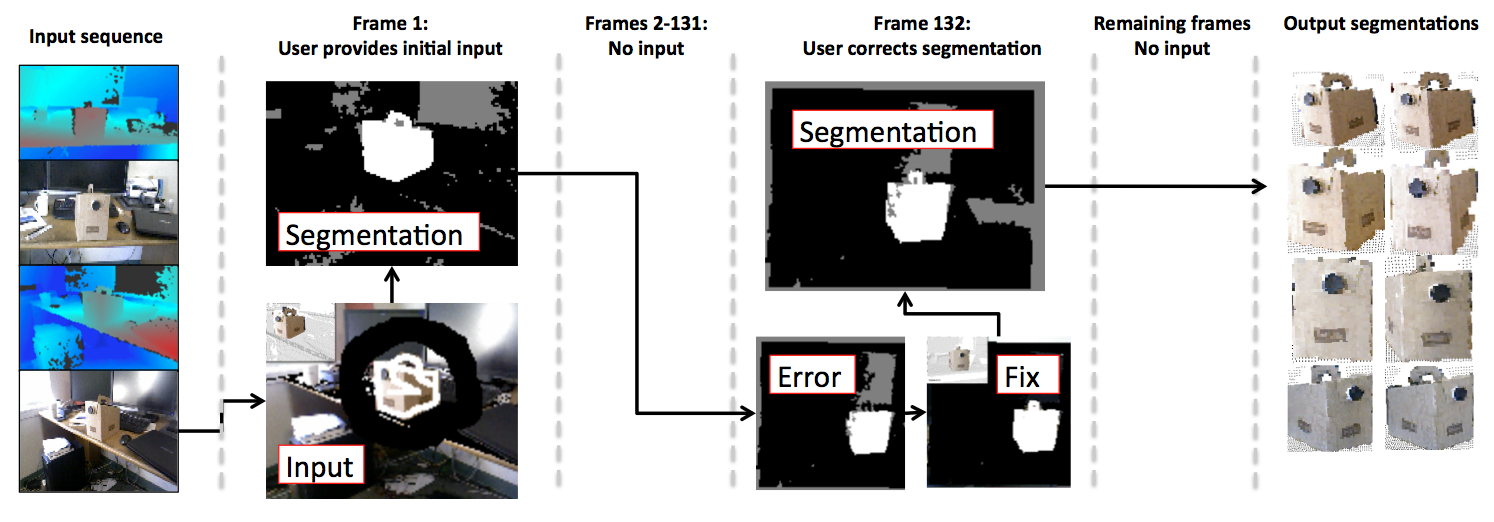
\includegraphics[width=\linewidth]{img/data_labeling.png}
\caption{\small{Example data labeling pipeline. Given an input RGBD sequence, the user first provides coarse, sparse foreground (white) and background (black) labels.  STRGEN properly segments subsequent frames until frame 132, at which point some minor corrections are required. STRGEN resumes and runs on the remaining 60 frames with no problems. The pipeline output is a set of clearly accurate object segmentations. }}
\label{fig:data_labeling}
\end{figure}

\begin{figure}
\centering
        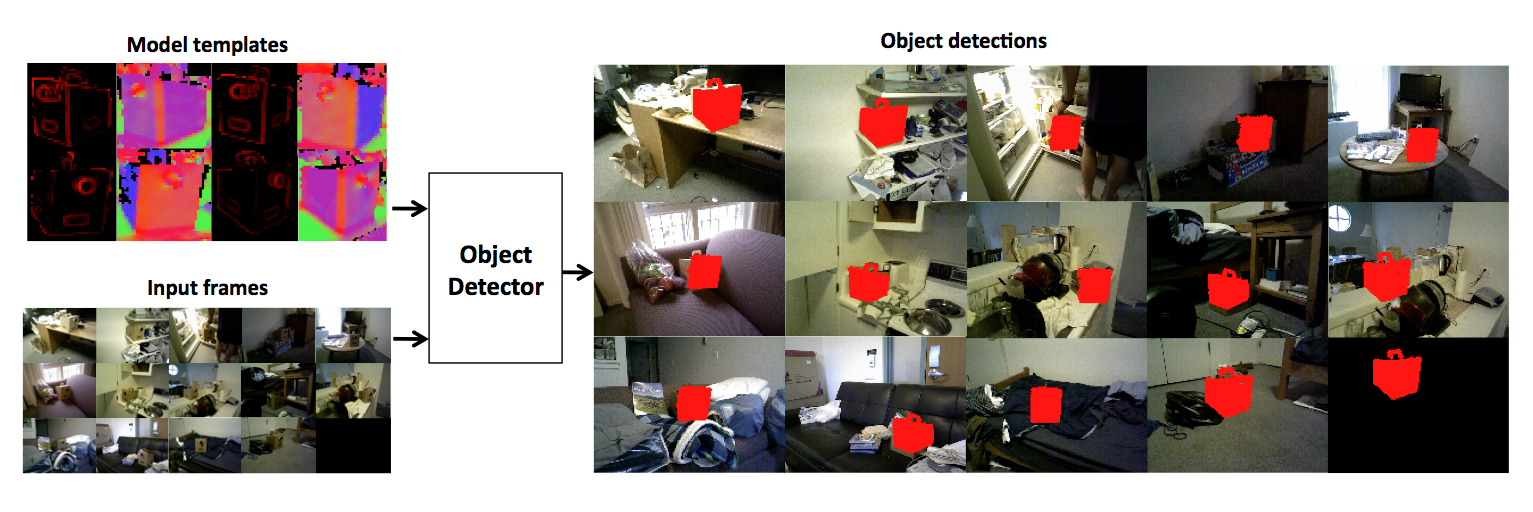
\includegraphics[width=\linewidth]{img/object_recognition.png}
\caption{\small{Object detection example. Color and depth templates are extracted from coffee box examples (such as those shown in Figure~\ref{fig:data_labeling}), and a set of unlabeled RGBD frames is provided.  An appropriate object detection method (LINE-MOD in our example) searches for the templates in the input frames and identifies the highest scoring match (shown in red). Note that given our cleanly segmented examples, LINE-MOD is able to accurately detect the object in 15 diverse scenes, under mild occlusion, and in different lighting levels (even in the absence of light in the last example). The detection with the highest response is taken in this example.}}
\label{fig:object_rec}
\end{figure}

\begin{figure}
\centering
        \includegraphics[width=\linewidth]{img/single_threshold.png}
\caption{\small{A second object detection example where all templates matches with responses $\ge 0.75$ are labeled detections. We register no false positives and effectively recover all object occurrences, even when there are multple or zero instances.}}
\label{fig:single_threshold}
\end{figure}

\section{Conclusions}

We have presented a novel method of segmenting and tracking deformable objects in RGBD, making minimal assumptions about the input data.  We have shown this method makes a significant quantitative improvement over the most similar state-of-the-art work in segmentation and tracking of non-rigid objects, that real-time performance is feasible, and that an online and interactive version of the algorithm is suitable for collecting training examples of objects in unstructured environments.  A complete solution to this task would have far-reaching ramifications in robotics, computer vision, and graphics, opening the door for easier-to-train and more reliable object recognition, model capture, and tracking-based semi-supervised learning.  While there remains more work to be done before a completely robust solution is available, we believe this approach to be a promising step in the right direction.

\pagebreak

\small{
\bibliographystyle{ieee}
\bibliography{tase2013}
}
\end{document}

This learning approach is essential to using a rich feature set, as hand-tuning the CRF weights is impractical.

Of those works that do consider this specific problem, none of them we are aware of use a learning approach to produce the best general-purpose tracker.


In contrast, we use a learning approach to intelligently combine a large number of features, including those derived from depth information.  No previous work we are aware of on this task uses learning in this way for the segmentation and tracking task.  Learning specific object models on the fly is common, but learning how to combine many diverse features to generate the most effective general-purpose segmentation and tracking model is new.


%  \caption{While image appearance and depth information may sometimes provide little information about on object boundary (for example, at the interface of a wooden object on a wooden table of the same color), a change in surface normals can be informative. Note this does not rely on any explicit ground plane detection but rather only local surface normal changes.  Surface normals are shown as small dark lines, seen from two angles to aid in depth perception.} 

  This presents a new problem: naively adding features corresponding to these intuitions without combining them in an intelligent way will generally result in a poor model.


In the past, rich and complex models that use many features were not possible to learn due to the intractability of computing the partition function present in computing the gradient.

Our approach relies on a conditional random field for capturing rich feature sets, graph cuts for efficient prediction of foreground/background labels, and structural SVMs for learning the relative importances of each of the terms in the energy function.


The goal is to segment and track an entire sequence correctly given a single seed frame.  However, this does not fit into the form required for efficient optimization via structural SVM, \ie predictions are required to be $\argmax_y w^T \Psi(y, x)$ for some unweighted feature function $\Psi(y, x)$; this is the case for segmenting a \emph{single} frame given the previous labeling, but the choice of $w$ affects $\Psi(y, x)$ on the next frame.  This is because features such as image appearance or frame-to-frame model fitting depend on the segmentation from the previous frame or frames.  To address this problem, we propose that the structural SVM learns the best parameters for segmenting the next frame assuming that all previous frames in the track have been segmented correctly.  This is important for correctly reasoning about potentials that accumulate state over the course of tracking.  For example, as the algorithm runs, each segmented frame is provided as training data to the patch classifier node potential.



A training set of thirteen ground-truth sequences, encompassing about 2400 frames, was labeled using the inference method of Section~\ref{sec:inference} using a rough guess for the parameters plus human labeling to correct errors.  Training was done once, and the final trained segmenter was used to generate all results.  All sequence labelings shown in this paper are from the test dataset and thus were not seen at training time.  All test sequences were given a single seed labeling at the first frame and no other input.

Unless otherwise specified, sequence numbers in the text are used to refer to sequences from Figure~\ref{fig:results} in order from top to bottom.


This method does not use the available depth information or apply learning to combine multiple feature types.

While we believe this direction to be a promising one, much work remains to be done.  The current implementation of the algorithm is still fragile when segmenting, for example, thin objects, quickly moving objects, and objects which frequently self-occlude parts. The current implementation also has no facility for re-acquiring targets after they have been lost.

Additionally, speedups of the node and edge potentials would be beneficial as faster framerates and higher resolutions result in better segmentations.  Node and edge potentials that explicitly reason about occlusion would also likely be useful.

eg \cite{kumar2011a}) viola2004a

\begin{align*}
  \phi_j(y, x) =
  \left\{
  \begin{array}{rl}
    0 & \mbox{ if } y_j = 1 \\
    -1 & \mbox{ if } y_j = -1.
  \end{array}
  \right.
\end{align*}


The remainder of this section discusses inference first, as it is a component of the learning algorithm, then learning, and finally the details of the energy function.

  The work of \cite{babenko2009a} applies multiple instance learning to the same task.



  \subsubsection{The importance of learning}

\begin{figure}
  \centering
  \includegraphics[width=\linewidth]{img/random.pdf}
  \caption{}
  \label{fig:random}
\end{figure}

Could probably use a method like this for learning, but it's incredibly slow.  This took overnight \todo{actual time?}, vs an average training time of 2.6 minutes for the structural SVM when using the boundary mask and 50\% downsampling of selected features, as described \todo{here}.  \todo{You could probably be smarter about caching for the random evaluations.  If you cached all the features for all frames, assuming the previous segmentation was correct, then evaluated random weights, you could avoid the vast majority of computation.  This would be at least an order of magnitude faster, possibly more.  That still might be an order of magnitude or two slower than structural SVM training, but without knowing this it's not fair to compare the running times and claim that random evaluation is too slow.  All you can claim here is that most random weights suck.   ... it might even be that with early termination (total error greater best error so far means you stop evaluating these weights) random evaluation turns out to be a reasonable method of learning. }


\begin{figure}
  \centering
  \includegraphics[width=0.3\linewidth]{img/front_and_back.pdf}
  \caption{A real-time interactive segmentation and tracking interface is used to collect labeled examples of a cat; the segmented object is shown with a red border (best viewed on-screen).  Using the methods in this paper, a system such as this one could be used for training robotic object recognition systems or 3D model capture in unstructured environments.}
  \label{fig:tricorder}
\end{figure}

and that no further information is provided other than the raw sensor data


Instead, we add a new node potential which biases these regions towards the label they had from the previous segmentation.


However, all these methods have at least one disadvantage such as a need for a calibrated data collection setup, slow collection rates, requirement of collecting data in a particular location, long turnaround time, quality control, or privacy issues.

This problem is slightly different from the STRGEN problem described above in that segmentation hints from a user are allowed at any time.

This same method could be used for 3D model-capture in unstructured environments, with all of the segmentation masks of a sequence being synthesized into one coherent object seen from all sides.

While the STRGEN algorithm of this paper cannot perfectly segment and track all objects, the presence of a human in the loop makes this method practical for the collection of training examples in unstructured environments; see 


the dataset includes rigid and non-rigid objects, and textured and non-textured objects.

While this is currently too slow for real-time usage, almost all of this time is spent computing features and only about a millisecond is spent on the graph cuts solver.  This means real-time performance can be achieved with speedups of feature computation alone, most immediately by parallelization and by computing features only at the boundaries of the object where they are actually needed.  At \vga resolution, graph cuts alone typically takes about 30ms; however, one could employ a similar trick and run the graph cuts solver only for the nodes near the boundaries of the object, providing a potentially large savings.
